\documentclass[conference,10pt]{IEEEtran}
\usepackage[utf8]{inputenc}
\usepackage{times}
\usepackage{graphicx}
\usepackage{booktabs}
\usepackage{amsmath}
\usepackage{url}
\usepackage[hidelinks]{hyperref}
\usepackage{xcolor}

\newcommand{\code}[1]{\texttt{\small #1}}
\newcommand{\cancollect}{\textsc{can-collect}}
\newcommand{\hascode}{\textsc{has-code}}
\newcommand{\observed}{\textsc{observed}}
\newcommand{\stored}{\textsc{stored-on-device}}

\begin{document}

\title{What the Apps Keep: An Evidence-Graded, Own-Device Study of Data Collection in TikTok and Xiaohongshu}

\author{\IEEEauthorblockN{Sreenandhu Nair}
\IEEEauthorblockA{Independent security research\\
\texttt{https://github.com/zkp6c4vr89-coder/tiktok-xhs-signing-analysis}}}

\maketitle

\begin{abstract}
Public debate about what mobile social apps collect is often muddied by conflating three very different claims: that an app \emph{could} collect something (a permission), that it \emph{has code} to collect it, and that it \emph{was seen} sending it. We study the Android apps of TikTok and Xiaohongshu (RedNote) and report every finding at exactly one of three strictly separated levels, plus a fourth for data persisted locally. All evidence comes from our own throwaway-account device; no bulk or automated requests are sent to either platform, and no raw personal values are published. Method aside, the sharpest result is about Xiaohongshu: its first-party API runs on a stripped Chromium Cronet stack that ignores the system proxy, and the app blocks the Frida Java bridge while native hooks still work, so first-party payloads are not observable with own-device instrumentation. What \emph{is} observable is substantial: on first launch and ordinary use the app contacts Facebook, AppsFlyer and Firebase, and it persists locally a per-note \emph{reading history with dwell time}, a full view history, and analytics queues whose zone defaults to \code{CN}. We release the evidence-graded field catalogue, permission and tracker tables, and the finding that Xiaohongshu resists own-device inspection on five independent layers. This paper is a companion to our earlier study of the same two platforms' request-signing code.
\end{abstract}

\section{Introduction}
Every few months a report claims a social app is ``spyware'' or, conversely, ``no worse than its peers.'' Both camps often lean on the weakest kind of evidence: a list of Android permissions. A permission means the app \emph{can} ask for data, not that it collects or sends it. Internet~2.0's widely-criticised TikTok report is the canonical example of reading ``has permission'' as ``is exfiltrating.'' The academic and NGO work is more careful. Citizen Lab's 2021 TikTok/Douyin study~\cite{citizenlab2021tiktok} is explicit that it is static source analysis and does not prove runtime transmission; its 2025 RedNote study~\cite{citizenlab2025rednote} is explicit that it is a \emph{network}-security analysis that did not assess first-party collection or government access; EFF's 2025 ``Crimson Memo''~\cite{eff2025crimson} confirmed those network findings. None of these claims to be a complete, graded picture of first-party collection.

This paper's contribution is a discipline, applied to two apps, and the data it produces. We grade every finding at one of three mutually exclusive levels, and keep a fourth for local persistence:

\begin{itemize}
  \item \cancollect{}: a permission is declared (manifest).
  \item \hascode{}: a collection or SDK code path is present (static).
  \item \observed{}: a value was actually seen on the wire (own-device dynamic capture).
  \item \stored{}: the app persists the data locally (own-device read of its data directory).
\end{itemize}

\noindent\textbf{Contributions.}
\begin{itemize}
  \item An evidence-graded field catalogue for TikTok 47.7.3 and Xiaohongshu 9.53.0, with each field pinned to a permission, a code location, a capture, or a local artifact, and the levels never conflated (Section~\ref{sec:method}).
  \item For Xiaohongshu, own-device \observed{} evidence of third-party SDK traffic and a \stored{} tier that includes a per-note reading history with dwell time and \code{CN}-defaulted analytics queues (Section~\ref{sec:xhs}).
  \item A documented account of \emph{why} first-party payloads resist capture: a five-layer hardening we verified by direct test, which extends the request-signing hardening reported in our companion paper (Section~\ref{sec:xhs},~\ref{sec:impact}).
  \item A reproducible, redaction-safe tooling pipeline that turns captures into field metadata without ever committing a raw value (Section~\ref{sec:method}).
\end{itemize}

\section{Background and Related Work}
Permissions, code, and transmission are three different things, and the literature that lasts keeps them apart. Citizen Lab's TikTok/Douyin analysis~\cite{citizenlab2021tiktok} examined Android source and found no overtly malicious behaviour, while noting Douyin-specific collection; it states plainly that static analysis does not establish what is sent at runtime. For Xiaohongshu, Citizen Lab~\cite{citizenlab2025rednote} found plaintext-HTTP media fetches and a TLS-without-validation flaw in the MobTech SDK, but scoped itself to network security and explicitly \emph{did not} assess first-party collection or state access; EFF~\cite{eff2025crimson} independently confirmed the network issues. Our work is complementary: we assess first-party and SDK collection from the device, graded by evidence strength, and we treat the China-access question the way the data supports it (Section~\ref{sec:impact}), not as proven transmission.

Our method rests on standard own-device dynamic analysis. We capture plaintext at the TLS boundary with Frida by hooking BoringSSL \code{SSL\_read}/\code{SSL\_write}, a long-standing technique, and we read the app's own data directory as root on an emulator. We do not use any flaw against anyone else's device.

\section{Method and Evidence Grading}
\label{sec:method}
\textbf{Pinned builds.} We analyse \code{com.zhiliaoapp.musically} 47.7.3 and \code{com.xingin.xhs} 9.53.0, both captured from APKMirror and pinned by SHA-256 in \code{data/apps.csv}. The copyrighted APKs and all raw captures stay git-ignored; findings are version-specific and current builds may differ.

\textbf{\cancollect{}.} We extract the declared permission set with \code{aapt2 dump permissions} and tabulate the dangerous/sensitive subset (\code{data/permissions\_*.csv}).

\textbf{\hascode{}.} We scan the DEX files for SDK namespaces and for the symbols of device-identifier collection APIs. A namespace or symbol reference is evidence that code exists, not that it runs; we label it so. We disambiguate real SDKs from lookalikes (for example, the Facebook \emph{SDK} via \code{FacebookSdk}/\code{login} classes, distinct from React Native's \code{com/facebook/*}).

\textbf{\observed{}.} On a rooted \code{android-34} emulator we install the mitmproxy CA into the system store, then capture plaintext by hooking \code{SSL\_read}/\code{SSL\_write} in the app process (reading our own pre-/post-encryption data). A redactor (\code{tools/dataflow/}) turns each captured request into \emph{field metadata only}: field name, a value \emph{shape} (type, length bucket, charset class), destination host, first-party-or-SDK, and a plaintext/encrypted heuristic. It never emits a raw value, treats any binary or compressed body as a single opaque field, and validates every field name as a token, so its output is safe to commit. A regression test asserts that no synthetic raw value can leak.

\textbf{\stored{}.} We read the app's own data directory on the emulator and record database \emph{schema} (table and column names) and shared-preference \emph{keys} only, never row values; the pulled databases stay git-ignored.

\textbf{Discipline.} The four levels are reported in separate columns and with separate verbs. ``Has permission'' and ``has code'' are never written as ``is sending.'' We treat any slip as a correctness bug. Figure~\ref{fig:tiers} shows the catalogue totals.

\begin{figure}[t]
  \centering
  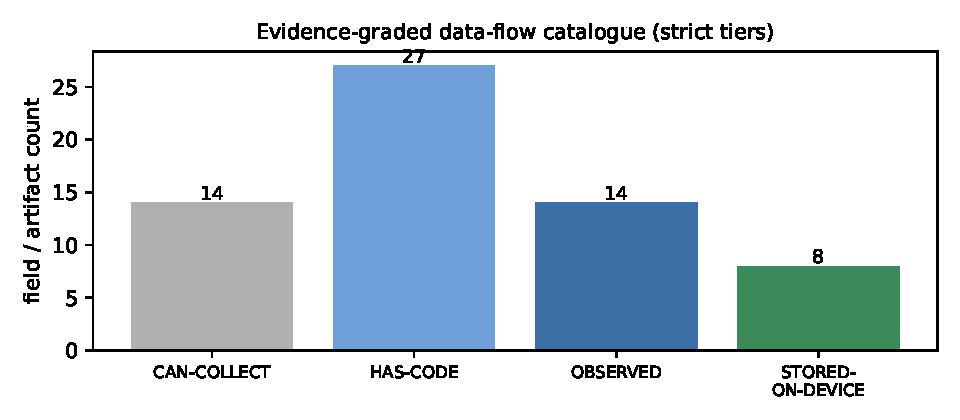
\includegraphics[width=\columnwidth]{figures/fig_tiers.pdf}
  \caption{The evidence-graded catalogue, counted by level. Each field or artifact is reported at exactly one level; lower levels are never promoted to higher ones.}
  \label{fig:tiers}
\end{figure}

\section{What TikTok Shows (static tiers)}
\label{sec:tiktok}
We report TikTok at the \cancollect{} and \hascode{} levels; its first-party API uses the same ByteDance/Cronet networking stack as Xiaohongshu (Section~\ref{sec:xhs}) and resists own-device capture for the same reasons, so we do not over-claim an \observed{} tier for it.

\textbf{\cancollect{}.} TikTok declares 64 permissions, 12 of them dangerous/sensitive, including precise and media location, contacts, microphone, camera, and Bluetooth scan/advertise (device-proximity) (Fig.~\ref{fig:perms}).

\textbf{\hascode{}.} The DEX references Google Firebase, Google Mobile Ads, AppsFlyer, the Facebook SDK, and Tencent SDKs, plus ByteDance's own first-party code; and it references collection APIs for the advertising ID, installed-app inventory, location, Wi-Fi MAC, contacts, clipboard, carrier/SIM, sensors, and device serial. Each is a code reference, not a traced live send.

\begin{figure}[t]
  \centering
  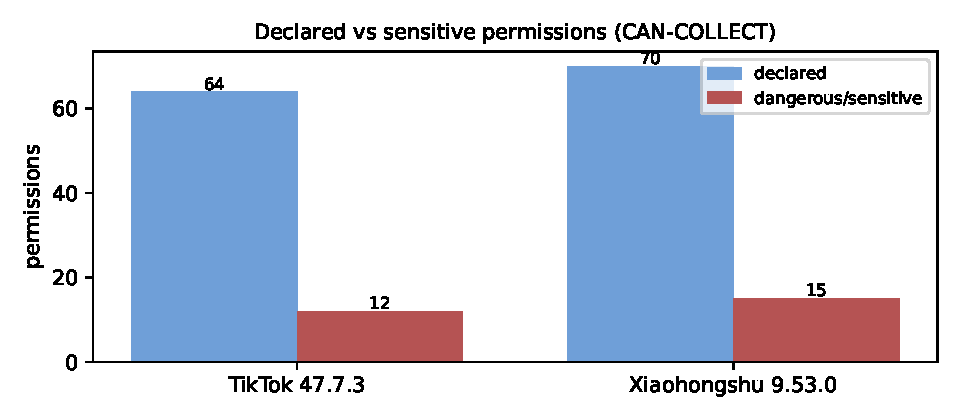
\includegraphics[width=\columnwidth]{figures/fig_perms.pdf}
  \caption{Declared versus dangerous/sensitive permissions (the \cancollect{} tier). Counts from \code{aapt2} on the pinned builds.}
  \label{fig:perms}
\end{figure}

\section{What Xiaohongshu Shows (all four tiers)}
\label{sec:xhs}
\textbf{\cancollect{}.} Xiaohongshu declares 70 permissions, 15 sensitive. Beyond the usual location/contacts/camera/microphone it declares calendar read/write and device-account access (\code{GET\_ACCOUNTS}/\code{MANAGE\_ACCOUNTS}), both less common.

\textbf{\hascode{}.} The same major SDKs as TikTok plus Alipay (payment) and AMap (maps/location). Notably, the clipboard-read API (\code{getPrimaryClip}) is referenced in eight DEX files, versus two in TikTok.

\textbf{\observed{}.} On first launch and ordinary use, hooking \code{SSL\_read}/\code{SSL\_write} captured plaintext traffic to third-party SDKs: \code{graph.facebook.com} (Facebook SDK: \code{access\_token}, \code{fields}, \code{platform}, \code{sdk}, \code{sdk\_version}), \code{appsflyersdk.com} (AppsFlyer: \code{app\_id}, \code{buildnumber}, an \code{androidevent} POST), and \code{firebaselogging.googleapis.com}. First-party hosts (\code{edith.rnote.com}, \code{edith.xiaohongshu.com}, the video/live CDN) were contacted, but their bodies are opaque (compressed/signed) and the signed feed/search/live API is not readable here (see hardening below). All values are redacted to shapes.

\textbf{\stored{}.} Reading the app's own data directory was the richest tier. Xiaohongshu persists locally (schema/keys only, values git-ignored; \code{data/stored\_on\_device\_xhs.csv}):
\begin{itemize}
  \item \code{NoteReadRecordDB.noteReadRecord} --- a per-note reading history with \emph{dwell time} (\code{stay\_seconds}), note id, title, timestamp.
  \item \code{PlayHistoryRecordDB.historyRecord} --- a full view history including \code{author\_id} and \code{user\_name}.
  \item \code{analysisemitter.sqlite} and \code{json\_tracker.apm} --- analytics event upload queues; \code{apm.zone} defaults to \code{CN}.
  \item \code{google\_app\_measurement\_local.db} --- a Firebase Analytics event queue.
  \item persistent identifiers in shared preferences: Facebook \code{anonymousAppDeviceGUID}, Firebase \code{app\_instance\_id}, AppsFlyer \code{AF\_INSTALLATION}/\code{attributionId}.
\end{itemize}
Local persistence is not the same as transmission; the analytics tables are explicitly upload \emph{queues}, which indicates intent but not, by itself, a send.

\textbf{Why first-party payloads resist capture (a finding).} We verified, by direct test, that Xiaohongshu resists own-device inspection on five independent layers (Table~\ref{tab:hardening}). The first-party API runs on Chromium Cronet (\code{libcronet.114.0.5735.38.so}), which ignores the system proxy and pins at a statically-linked, fully-stripped BoringSSL (zero \code{SSL\_*} symbols). The app uses Cronet's Java/JNI path, so the exported Cronet C-API functions we hooked never fire. And the Frida Java bridge never initialises in the app process, although native hooks work, so Java-layer hooks cannot be installed. The remaining theoretical paths cross from reading our own data into defeating the app's protections, which is out of scope. This mirrors, from the app side, the request-signing hardening in our companion paper.

\begin{table}[t]
\caption{Own-device methods tried to read Xiaohongshu's first-party payloads, and why each stops. Native hooks work; Java and Cronet-plaintext paths do not.}
\label{tab:hardening}
\centering\footnotesize
\resizebox{\columnwidth}{!}{%
\begin{tabular}{@{}p{0.52\columnwidth}p{0.46\columnwidth}@{}}
\toprule
Method & Result \\
\midrule
HTTP proxy (mitmproxy) & Cronet ignores system proxy \\
Native \code{SSL\_*} by symbol & Only non-Cronet TLS (SDK, media) \\
\code{libcronet} BoringSSL symbol & Fully stripped (0 symbols) \\
Cronet C-API hook & Installs, never fires (Java path) \\
Frida Java hooks & \code{Java} never available (anti-tamper) \\
\bottomrule
\end{tabular}}
\end{table}

\section{Individual Impact}
\label{sec:impact}
\textbf{Fingerprinting and identifiers.} Both apps' \hascode{} tier references the advertising ID, installed-app inventory, carrier, sensors, and serial; Xiaohongshu's \stored{} tier shows persistent cross-SDK identifiers (Facebook device GUID, Firebase instance id, AppsFlyer installation id). These are the building blocks of stable device identification.

\textbf{Cross-app linkage.} The same three advertising/analytics SDKs (Facebook, AppsFlyer, Firebase) appear in both apps and were \observed{} receiving data from Xiaohongshu. Shared SDK identifiers are a known mechanism for linking a person across unrelated apps.

\textbf{Behavioural profiling.} The \stored{} reading history with \code{stay\_seconds} is a fine-grained record of attention (which notes, how long). That is a stronger behavioural signal than a simple view log.

\textbf{Network surveillance.} Consistent with Citizen Lab~\cite{citizenlab2025rednote}, some content is reachable by a network observer; our capture also shows media/live-CDN content identifiers in plaintext.

\textbf{Jurisdiction.} Xiaohongshu is operated from mainland China and its on-device analytics queue defaults to a \code{CN} zone. We state the access question precisely: the operator is \emph{subject to laws that could compel disclosure} of data it holds. We did \emph{not} observe first-party data being transmitted to any specific destination (it is Cronet-opaque), and we do not claim such transmission as proven.

\section{Ethics and Scope}
This is defensive, educational research with no affiliation to either company. Four rules bound it. (1)~\emph{Own device only}: all captures are from a throwaway account on an emulator we control, used at human pace; we sent no automated or bulk requests to either platform, and this is not a scraper. (2)~\emph{No raw personal data}: we publish field names, value shapes, destination hosts, SDK attribution, and plaintext/encrypted status, never our real values; raw captures and databases stay git-ignored, and the redactor is tested to prevent leaks. (3)~\emph{No attacking others}: we did not use the MobTech certificate-validation flaw against any device, did not decrypt anyone else's data, and did not forge requests. Reading our own outbound data is in scope; disabling a hardened app's integrity or anti-tamper protections is not, which is why the Xiaohongshu first-party \observed{} tier stops where it does. (4)~\emph{No invented results}: every field traces to a capture file or code location in the repository, and every cited work was verified to exist.

\section{Limitations}
Findings are pinned to two specific builds and will drift. The \observed{} tier is asymmetric: we captured Xiaohongshu's SDK traffic but not its Cronet first-party payloads, and we did not attempt a TikTok dynamic capture because it uses the same resistant stack. \hascode{} rows are code references, not traced live calls. \stored{} rows show local persistence, not transmission. The tracker list is namespace-based, not a full Exodus classification. The emulator and anti-tamper interactions were occasionally unstable. These gaps are disclosed rather than hidden, and the hardening that produces them is itself reported as a result.

\section{Conclusion}
Graded honestly, the two apps look different from either the ``spyware'' or the ``nothing to see'' headline. At the levels the evidence supports, both can and do integrate the major advertising/analytics SDKs, and Xiaohongshu keeps a detailed, dwell-time reading history on the device with analytics queued to a \code{CN} zone. The first-party network payloads that would complete the picture are deliberately placed beyond own-device observation by a five-layer hardening, the same engineering posture our companion paper found in these platforms' request-signing code. The contribution here is not a single alarming number but a method that refuses to conflate ``could,'' ``has code,'' ``was seen,'' and ``is kept.''

\appendices
\section{Catalogue and Tables}
The full artifacts are in the repository: the evidence-graded field catalogue (\code{data/field\_catalogue.csv}); the \stored{} tier (\code{data/stored\_on\_device\_xhs.csv}); per-app permission tables (\code{data/permissions\_*.csv}); the tracker/SDK list (\code{data/trackers.csv}); pinned builds (\code{data/apps.csv}); and per-app notes (\code{analysis/\{tiktok,xhs\}/dataflow.md}).

\begin{thebibliography}{9}
\bibitem{citizenlab2021tiktok} P.~Lin, ``TikTok vs Douyin: A Security and Privacy Analysis,'' The Citizen Lab, Univ.\ of Toronto, Mar.\ 2021.
\bibitem{citizenlab2025rednote} M.~Wang, J.~Knockel, and I.~Poetranto, ``Network Security Issues in RedNote,'' The Citizen Lab, Univ.\ of Toronto, Feb.\ 2025.
\bibitem{eff2025crimson} Electronic Frontier Foundation, ``Crimson Memo: Analyzing the Privacy Impact of Xiaohongshu AKA Red Note,'' Feb.\ 2025.
\bibitem{paper1} S.~Nair, ``Client-side Request Signing on TikTok and Xiaohongshu Web: a Reproducible Study,'' 2026. Companion paper.
\end{thebibliography}

\end{document}
